%%「論文」,「レター」,「レター(C分冊)」,「技術研究報告」などのテンプレート
%% 1. 「論文」
%% v1.6 [2009/11/03]
\documentclass{ieicej}
%\documentclass[invited]{ieicej} % 招待論文
%\documentclass[comment]{ieicej} % 解説論文
\usepackage{graphicx}
%\usepackage{latexsym}
\usepackage[fleqn]{amsmath}
\usepackage{amsfonts}
\usepackage[psamsfonts]{amssymb}

\setcounter{page}{1}

\field{}
\jtitle{二重値付き時間オートマトンを用いた\\非停止スケジューリングにおける最適平均利得計算の実現}
\etitle{An Inplementation of Computing Optimal Mean-payoff Values for \\Non-terminating Scheduling by Double Priced Timed Automata}
\authorlist{%
 \authorentry{平岡 祥}{Sho HIRAOKA}{Nagoya}% <= 記述しないとエラーになります
 %\authorentry{和文著者名}{英文著者名}{所属ラベル}
 %\authorentry[メールアドレス]{和文著者名}{英文著者名}{所属ラベル}
 %\authorentry{和文著者名}{英文著者名}{所属ラベル}[現在の所属ラベル]
}
\affiliate[Nagoya]{名古屋大学大学院情報科学研究科,名古屋市}{}
%\affiliate[所属ラベル]{和文所属}{英文所属}
%\paffiliate[]{}
%\paffiliate[現在の所属ラベル]{和文所属}

\begin{document}
\begin{abstract}
%和文あらまし 500字以内
本研究では提案したアルゴリズムに基づくツールを実装して,いくつかのサンプルを与えアルゴリズムの各段階における実行時間を評価した.
\end{abstract}
\begin{keyword}
%和文キーワード 4〜5語
\end{keyword}
\begin{eabstract}
%英文アブストラクト 100 words
We implement a optimization tool using the proposed algorithm and evaluated the execution time of each stage of the algorithm by giving some samples.
\end{eabstract}
\begin{ekeyword}
%英文キーワード
\end{ekeyword}
\maketitle

\section{まえがき}
%研究の目的
実時間システムは,与えられたタスクの処理をデッドラインを超えないように動作する.
スケジュール可能性に加えて,実行に対して量的な解析を行うことによって実時間システムをより効率的に動作させることが可能になる.
ここでは,スケジューラが与えられたタスクに対して,どの程度効率的に動作するかを定量的にモデル化することにより,複数のスケジューリングに対して効率の大小を定義することができるようになる.
例えば処理できるタスクが最多となるスケジューリングや処理時間が最も短くなるようなスケジューラはより適切であるといえる.

%従来のモデルではそもそも実時間システムは解析できない
このような解析を行うために,従来の離散的な状態遷移に加えて連続的な時間経過に応じて変化する量を扱えるモデルを用いる必要がある.

%時間を扱ったモデルならば質的な解析ができる
時間を扱えるモデルは既にいくつか研究されている.
例えば時間オートマトン\cite{ta}は有限オートマトンの拡張であり,システムを不連続なイベントと連続的な時間経過の両方による状態遷移で記述したモデルである.

%時間と時間に依存した量を扱ったモデルならば量的な解析ができる
スケジューラの量的な解析を行うには値付き時間オートマトン\cite{pta}を用いる.
値付き時間オートマトンは時間オートマトンの拡張であり,決定可能性を保ちながら時間と時間に依存する量を扱うことができるモデルである.
例えば,時間に依存する量の例としてメモリが挙げられる.
メモリの場合は,消費量が少なければ少ないほど適切な振る舞いであると言える.
この拡張によって,時間オートマトンの受理する有限長の語に対応した振る舞いに対して量的な解析を行うことが可能になる.

%量的な解析をOSに応用したい
しかしOSのような停止しないスケジューラの振る舞い解析において,値付き時間オートマトンでは時間経過とともに増加する値に対して,有限長の受理後による量的な解析をすることができない.
そこで,停止しないシステムを扱うために二重値付き時間オートマトン\cite{dpta}を用いる.
二重値付き時間オートマトンは値付き時間オートマトンの拡張であり,時間に依存する量を2個保持し,増加の割合を表現することができる.
時間に依存する値が二つあるため,二つの時間に依存する値の比をとることで無限の動作に対しても量的な解析が可能である.
二つの値の比である利得によって実行効率をモデル化し,利得の最小化によってスケジューリングの効率化の最適性を示す.

%やったこと
二重値付き時間オートマトンを用いて無限に動作するスケジューリングの最適な利得が導出可能であることは既存研究\cite{dpta}によって示されているが,最適な利得を導出する具体的なアルゴリズムは示されていない.
本研究では最適な利得を導出するアルゴリズムを示し,具体的なアルゴリズムに基づくツールを実装して最適平均利得を導出する.
また,いくつかのサンプルを与えアルゴリズムの各段階における実行時間や状態数を評価する.

%構成
本論文の構成は以下の通りである.
第2章では,準備として二重値付き時間オートマトンの定義や最適平均利得の計算可能性について述べる.
第3章では,最適平均利得を導出するアルゴリズムについて述べる.
第4章では,第3章で提案したアルゴリズムを基に実装したツールの実行時間や状態数を評価する.
第5章では,まとめと今後の課題を述べる.




\section{二重値付き時間オートマトン}
\subsection{定義}
%トランジションシステムは時間経過をトランじしょんとして表している.
%ハイブリットオートマトンなので連続的なトランジションしているときはあるロケーションでじっとしている.
%あるとき次のロケーションへ移る.
%ディスクリートなトランジションはいいけど連続的なやつはこのシステムで考える.
%コストやリウォードが→にだけ割り当てられている.
%直接書くとすると状態というのをDPTSで書く.
%Sにはクロックアサインメントが埋め込まれている.
%Sというのをロケーションと.μはクロックを与えると関数のペアで書けばかける.
%sはロケーションとクロックの値(のベクトル)

二重値付き時間オートマトンは,時間オートマトンに時間に依存する2つの量を加えた状態遷移システムのモデルである.
時間オートマトンは有限オートマトンの拡張であり,時間を扱うことができる.
時間には非負実数を,時間制約は自然数を用いる.
有限オートマトンのロケーションにインバリアントを追加し,エッジにガードとリセットを追加する.
インバリアントはロケーションにとどまることが可能な時間である.
クロックがガードを満たすとき遷移が可能であり,遷移にリセットがあれば指定されたクロックを初期化する.

二重値付き時間オートマトンでは,ロケーションとエッジにコストとリウォードを追加する.
ロケーションにコストとリウォードの単位時間あたりの増加量を記述し,エッジにコストとリウォードの遷移するときの増加量を記述する.

以下に二重値付き時間オートマトンの定義を示す.

\newtheorem{teiri}{定理}
\begin{teiri}
	クロックの有限集合$X$上のクロック制約式$g$の構文を以下のように与える.

%	\begin{center}
		$g ::= x \bowtie c \; | \; g \wedge g \; (x \in X, c \in \mathbb{N}, \bowtie \; \in \{<, \leq , =, \geq , >\})$
%	\end{center}
	
	ここで,$\mathcal{C}(X)$を$X$上のクロック制約式$g$からなる集合とする.
\end{teiri}

%\begin{definition}
	$X$上で動作する二重値付き時間オートマトン$\mathcal{A}$は6項組$(L, l_0, E, I, c, r)$で与えられる.
	\begin{description}
%		\begin{indentation}{2zw}{0zw}
			\item [$L$:] ロケーションの集合.
			\item [$l_0$:] 初期ロケーション.
			($l_0 \in L$)
			\item [$E $:] エッジの集合.
			エッジは遷移前のロケーション,ガード,リセット,遷移後のロケーションからなる.
			($E \subseteq L \times \mathcal{C}(X) \times 2^X \times L$,($l, g, Y, l'$)$\in E$のとき$l \xrightarrow[]{g, Y} l'$と記述する)
			\item [$I$:] ロケーションのインバリアント.
			($I : L \rightarrow \mathcal{C}(X)$)
			\item [$c$:] ロケーションにおけるコストの増加量,またはエッジにかかるコスト.
			($c : (L \cup E) \rightarrow \mathbb{Z}$)
			\item [$r$:] ロケーションにおけるリウォードの増加量,またはエッジにかかるリウォード.
			($r : (L \cup E) \rightarrow \mathbb{Z}$)
%		\end{indentation}
	\end{description}
%\end{definition}

%二重値付き時間オートマトンの例を図\ref{fg:example21}に示す.

\begin{figure}[tb]
	\begin{center}
		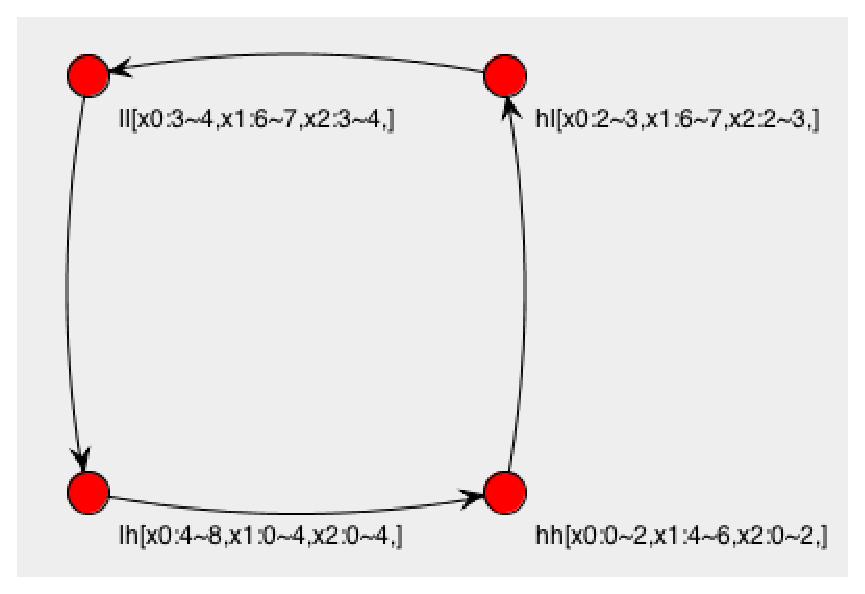
\includegraphics[width=50mm]{images/optimal.eps}
		\caption{二重値付き時間オートマトンの例}
		\label{fg:example21}
	\end{center}
\end{figure}

図\ref{fg:example21}の二重値付きオートマトンの初期ロケーションはHighである.
Highにいる間はコストが単位時間あたり3,リウォードは単位時間あたり4増加する.
Highのインバリアントが$x \leqq 3$であるため,クロック$x$が3より大きくなる前にはLowに遷移する.
HighからLowへのエッジにはガードがないため,$0 \leqq x \leqq 3$の間ならばLowへ遷移できる.

Lowにいる間はコストが単位時間あたり3,リウォードは単位時間あたり2増加する.
Lowにインバリアントはないため,$x$の値に関わらずLowに滞在可能である.
LowからHighへのエッジのガードが$x \geqq 4$であるため,LowからHighへの遷移は$x$が4以上のときに可能である.
リセットが$x := 0$であるため,LowからHighへの遷移時に$x$を0にする.
また遷移したときにコストが3,リウォードが4増加する.

コストの累計をリウォードの累計で割った比を利得と呼ぶ.
システムの動作を量的に評価するとき,利得が基準となる.
利得はできるだけ小さい方が良い.
図\ref{fg:example21}の例において,Highのコストとリウォードの増加量の比は$3/4 = 0.75$,Lowのコストとリウォードの増加量の比は$5/2 = 2.5$であるため,できるだけHighに居続けることが望ましい.



%\section{コストとリウォードによるスケジューリングの平均利得}
%振動するときにすんなり収束するわけではなく振動のしたべり(最小のとこ)をとってって回数が進んでったときに一番最小なところとってくる.



\subsection{コーナーポイント抽象化による最適平均利得の計算可能性}
%コーナーポイントアブストラクションをすると有限に落ちるというとこ.
%時間が連続なので.連続は計算機では扱えないが有理数は稠密(でんす)なので扱える.
%それが無限にあるのでその中のコーナーポイントだけやればよい.
%微分してやるやつの話.
%ACMの解説論文の方がわかりやすい.
二重値付き時間オートマトンの全ての閉路を一周した際に得られる利得のうち,最小となる利得を最適平均利得と呼ぶ.
最適平均利得を求めるには二重値付き時間オートマトンの解析を行う必要があるが,二重値付き時間オートマトンにおける時間は実数値であるため状態の数が無限となる.
%無限ではダメな理由.モデル検査が
計算機で解析を行うためには有限状態に変換する必要がある.
そこで,リージョン抽象化\cite{ta}とコーナーポイント抽象化\cite{pta}を用いる.

リージョン抽象化は時間オートマトンを有限状態に変換する手法である.
リージョン抽象化では遷移の可否に影響しないようなクロック変数の付値の違いを無視することで,付値の集合をリージョンと呼ばれる部分集合に分割する.
リージョン中ではクロックの整数の値は変わらないため,時間オートマトンの振る舞いは変わらない.
クロックがガードかインバリアントに現れる最大の整数を超えたときは時間オートマトンの振る舞いには影響を与えないため,リージョンに分割できる.
クロック制約に出現する最大の整数を$M$とする.

%一般的な分割,単位時間ごとに分ける
%\begin{definition}
	リージョンは$r=(h, [X_0, ..., X_p])$で与えられる.($p$は整数)
	\begin{description}
%	\begin{indentation}{2zw}{0zw}
		\item [$h$:] クロックの整数部分.($h:X \rightarrow \mathbb{N} \cap [0, M]$)
		\item [$(X_i)_{i=0, ..., p}$:] クロックの大小関係を示すパーティション.($i > 0$ならば$X_i \neq \phi$であり,$h(x) = M$ならば$x \in X_0$である)
%	\end{indentation}
	\end{description}
%\end{definition}

$v$が与えられたとき,$v$は以下のようにしてリージョン$r$にいると言える.
\begin{itemize}
	\item あるクロック$x \in X$に対して,$v(x)$の整数部分は$h(x)$となる.
	\item あるクロック$x \in X$に対して,$x \in X_0 \Longleftrightarrow v(x) = h(x)$.
	\item 全てのクロック$(x, y)$に対して,$\langle v(x)\rangle \leqq \langle v(y)\rangle \Longleftrightarrow x \in X_i$かつ$y \in X_j$.($i \leqq j$,$\langle・\rangle$は小数部分を表す)
\end{itemize}


例として$X=\{x, y\}$,$M=2$であるとき,リージョンは図\ref{fg:region}のようになる.

\begin{figure}[htbp]
	\begin{center}
%		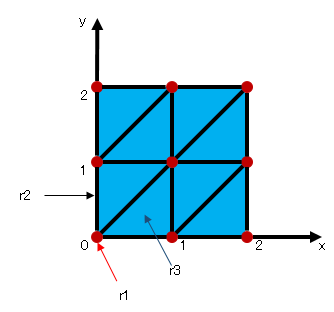
\includegraphics[width = 7cm]{images/region.png}
		\caption{$X=\{x, y\}$, $M=2$であるリージョン概略図}
		\label{fg:region}
	\end{center}
\end{figure}

リージョンは以下のように分割される.

\begin{enumerate}
	\item 2変数とも整数.
	グラフ上では点で示される.
	(図\ref{fg:region}における赤色の部分)
	(例:$r1 = (h, [X_0 =\{x, y\}]) $)
	\item 片方の変数のみ整数,または2変数の小数の値が同じ.
	グラフ上では線で示される.
	(図\ref{fg:region}における黒色の部分)
	(例:$r2 = (h, [X_0 =\{x\}, X_1=\{y\}]) $)
	\item 1,2に当てはまらず,2変数ともクロック制約の最大値を超えていない.
	グラフ上では三角形で示される.
	(図\ref{fg:region}における青色の部分)
	(例:$r3 = (h, [X_0 =\{\}, X_1=\{y\}, X_2=\{x\}]) $)
\end{enumerate}



二重値付き時間オートマトンは時間に依存する値であるコストやリウォードを持ち,同じリージョンでもコストやリウォードの値が異なるため,リージョン抽象化では有限状態へ変換することができない.
そこで,コーナーポイント抽象化を用いることで二重値付き時間オートマトンを有限状態へ変換する.

%コーナーポイントに分ける理由
%リージョン抽象化ではコストやりうx−どの値の違いを考慮していない
%そこでコーナーポイント抽象化を使うことで
コーナーポイント抽象化では,リージョン抽象化によって分けられたリージョンを更にコーナーポイントと呼ばれる部分集合に分割する.
リージョン内で利得が最小となる可能性があるのはクロックが整数値をとる場合のみであるため,リージョン内のクロックのうち,整数値であるコーナーポイントを考える.
%リージョンのパーティションにおけるiで切り上げ切り下げをする.
%\begin{definition}
	コーナーポイントは$\alpha = (a_j)_{1\leqq j \leqq k}$で与えられる($k$はクロック数).全ての$j$($1 \leqq j \leqq k$)に対し,$a_j$は$0 \leqq a_j \leqq M$の整数となる.
%\end{definition}

リージョン$r=(h, [X_0, ..., X_p])$は$p+1$個のコーナーポイント$(\alpha_i)_{0 \leqq i \leqq p}$に分割され,$\alpha_i$は以下のように定義される.

\begin{equation}
	\alpha_i(x) = \left \{
	\begin{array}{l}
		h(x)\:\:\:\:\:\:\:\:\:(x \in X_j かつ j \leqq iの場合) \\
		h(x)+1(x \in X_j かつ j > iの場合)
	\end{array}
	\right.
\end{equation}

%\begin{definition}
	有限状態の遷移システム$\mathcal{A}_{cp} = (S, s_0, T, cost, reward)$を与える.($\mathcal{A}_{cp}$は二重値付き時間オートマトン$\mathcal{A}$をコーナーポイント抽象化したもの)
	\begin{description}
%	\begin{indentation}{2zw}{0zw}
		\item [$S$:] 状態の集合.
		\item [$s_0$:] 初期状態.($s_0 \in S$)
		\item [$T$:] 遷移の集合.($T \subseteq S \times S$)
		\item [$cost$:] 遷移におけるコストの増加量.($cost:T \rightarrow \mathcal{R}$)
		\item [$reward$:] 遷移におけるコストの増加量.($reward:T \rightarrow \mathcal{R}$)
%	\end{indentation}
	\end{description}
%\end{definition}

$\mathcal{A}_{cp}$の状態($\in S$)は($l, R, \alpha$)の形で記述される.
$l$はロケーションであり,$R$はリージョン,$\alpha$はコーナーポイントである.
$\mathcal{A}_{cp}$の遷移($\in T$)は以下のように定義される

\begin{description}
	\item [二重値付き時間オートマトンの遷移に対応するコーナーポイントの遷移] \mbox{} \\
		$\mathcal{A}$の遷移$e = l \xrightarrow[]{g, Y} l'$は,$\mathcal{A}_{cp}$において$e' = (l, R, \alpha) \rightarrow (l', R', \alpha )$となる.
		リセット$Y$に含まれるクロック変数$x$について,$x$を$X_i$から取り除き$X_0$に追加したものを$R'$とする.		
		また,$\alpha(x) = 0$とする.
		コストとリウォードは二重値付き時間オートマトンの遷移におけるコストとリウォードと同値である.
	\item [同じロケーションでの時間経過による遷移] \mbox{} \\
		\begin{itemize}
			\item 現状態において$\alpha = \alpha_p$かつ$X_0 = \{ \phi \}$の場合,$e' = (l, R, \alpha) \rightarrow (l, R, \alpha' )$とし,$\alpha'$は$\alpha$の全ての要素を1増加したものとする.
			\item $\alpha \neq \alpha_p$もしくは$X_0 \neq \{ \phi \}$の場合,図\ref{fg:corner_point}のように隣接したリージョン$R,R'$について$e' = (l, R, \alpha) \rightarrow (l, R', \alpha)$とする.
		\end{itemize}
\end{description}

\begin{figure}[htbp]
	\begin{center}
%		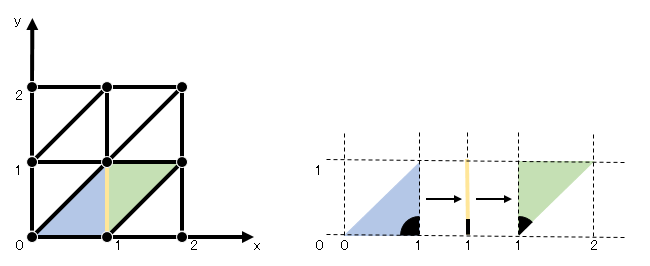
\includegraphics[width = 15cm]{images/corner_point.png}
		\caption{隣接するコーナーポイントの遷移}
		\label{fg:corner_point}
	\end{center}
\end{figure}

%リージョン内で利得が最小となる可能性があるのはクロックが整数値をとる場合のみである.


最適平均利得を考える際,利得が最小となるような振る舞いを選ぶ.
クロック制約が整数の範囲で記述されているため,利得が最小となる可能性があるのはクロックが整数値をとる場合のみである.
よって,コーナーポイント抽象化によって最適平均利得を計算することが出来る.



\ack %% 謝辞

%\bibliographystyle{sieicej}
%\bibliography{myrefs}
\begin{thebibliography}{99}% 文献数が10未満の時 {9}
\bibitem{}
\end{thebibliography}

\appendix
\section{}

\begin{biography}
\profile*{s}{平岡 祥}{}
%\profile{会員種別}{名前}{紹介文}% 顔写真あり
%\profile*{会員種別}{名前}{紹介文}% 顔写真なし
\end{biography}

\end{document}



%% 2. 「レター」
\documentclass[letter]{ieicej}
\usepackage{graphicx}
%\usepackage{latexsym}
%\usepackage[fleqn]{amsmath}
%\usepackage[psamsfonts]{amssymb}

\setcounter{page}{1}

\typeofletter{研究速報}
%\typeofletter{紙上討論}
%\typeofletter{問題提起}
%\typeofletter{ショートノート}
\field{}
\jtitle{}
\etitle{}
\authorlist{%
 \authorentry{a}{b}{c}{d}% <= 記述しないとエラーになります
 %\authorentry{和文著者名}{英文著者名}{会員種別}{所属ラベル}
 %\authorentry{和文著者名}{英文著者名}{会員種別}{所属ラベル}[現在の所属ラベル]
}
\affiliate[]{}{}
%\affiliate[所属ラベル]{和文所属}{英文所属}
%\paffiliate[]{}
%\paffiliate[現在の所属ラベル]{和文所属}

\begin{document}
\maketitle
\begin{abstract}
%和文あらまし 120字以内
\end{abstract}
\begin{keyword}
%和文キーワード 4〜5語
\end{keyword}
\begin{eabstract}
%英文アブストラクト 50 words
\end{eabstract}
\begin{ekeyword}
%英文キーワード
\end{ekeyword}

\section{まえがき}
やっほー.
\subsection{たかし}
\section{あとがき}


\ack %% 謝辞

%\bibliographystyle{sieicej}
%\bibliography{myrefs}
\begin{thebibliography}{99}% 文献数が10未満の時 {9}
\bibitem{}
\end{thebibliography}

\appendix
\section{}

\end{document}


%% 3. 「レター(C分冊)」
\documentclass[electronicsletter]{ieicej}
\usepackage{graphicx}
%\usepackage{latexsym}
%\usepackage[fleqn]{amsmath}
%\usepackage[psamsfonts]{amssymb}

\setcounter{page}{1}

\field{}
\jtitle{}
\etitle{}
\authorlist{%
 \authorentry{a}{b}{c}{d}% <= 記述しないとエラーになります
 %\authorentry{和文著者名}{英文著者名}{会員種別}{所属ラベル}
 %\authorentry{和文著者名}{英文著者名}{会員種別}{所属ラベル}[現在の所属ラベル]
}
\affiliate[]{}{}
%\affiliate[所属ラベル]{和文所属}{英文所属}
%\paffiliate[]{}
%\paffiliate[現在の所属ラベル]{和文所属}

\begin{document}
\begin{abstract}
%和文あらまし 120字以内
\end{abstract}
\begin{keyword}
%和文キーワード 4〜5語
\end{keyword}
\begin{eabstract}
%英文アブストラクト 50 words
\end{eabstract}
\begin{ekeyword}
%英文キーワード
\end{ekeyword}
\maketitle

\section{まえがき}


\ack %% 謝辞

%\bibliographystyle{sieicej}
%\bibliography{myrefs}
\begin{thebibliography}{99}% 文献数が 10 未満の時 {9}
\bibitem{}
\end{thebibliography}

\appendix
\section{}

\end{document}



%% 4. 「技術研究報告」
\documentclass[technicalreport]{ieicej}
\usepackage{graphicx}
%\usepackage{latexsym}
%\usepackage[fleqn]{amsmath}
%\usepackage[psamsfonts]{amssymb}

\jtitle{}
\jsubtitle{}
\etitle{}
\esubtitle{}
\authorlist{%
 \authorentry[a]{b}{c}{d}% <= 記述しないとエラーになります
% \authorentry[メールアドレス]{和文著者名}{英文著者名}{所属ラベル}
}
\affiliate[]{}{}
%\affiliate[所属ラベル]{和文勤務先\\ 連絡先住所}{英文勤務先\\ 英文連絡先住所}

\begin{document}
\begin{jabstract}
%和文あらまし
\end{jabstract}
\begin{jkeyword}
%和文キーワード
\end{jkeyword}
\begin{eabstract}
%英文アブストラクト
\end{eabstract}
\begin{ekeyword}
%英文キーワード
\end{ekeyword}
\maketitle

\section{はじめに}


%\bibliographystyle{sieicej}
%\bibliography{myrefs}
\begin{thebibliography}{99}% 文献数が10未満の時 {9}
\bibitem{}
\end{thebibliography}

\end{document}
